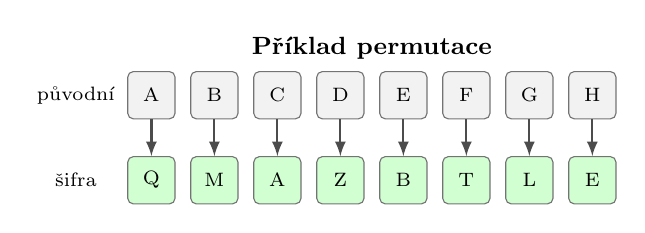
\begin{tikzpicture}[
    x=0.8cm, y=0.8cm,
    >=latex,
    cell/.style={
        draw=black!55,
        rounded corners=0.7mm,
        minimum width=0.6cm,
        minimum height=0.6cm,
        font=\scriptsize
    },
    arrow/.style={
        ->,
        line width=0.8pt,
        draw=black!70
    }
]

    \foreach \x/\letter in {
        0/A,1/B,2/C,3/D,4/E,5/F,6/G,7/H
    }{
        \node[cell, fill=black!5] (u\x) at (\x,0) {\letter};
    }

    \foreach \x/\letter in {
        0/Q,1/M,2/A,3/Z,4/B,5/T,6/L,7/E
    }{
        \node[cell, fill=green!18] (d\x) at (\x,-1.35) {\letter};
    }

    \foreach \x in {0,1,2,3,4,5,6,7}{
        \draw[arrow] (u\x) -- (d\x);
    }

    \node[font=\scriptsize] at (-1.2,0) {původní};
    \node[font=\scriptsize] at (-1.2,-1.35) {šifra};

    \node[font=\small\bfseries] at (3.5,0.75)
        {Příklad permutace};

\end{tikzpicture}
